\documentclass[11pt, twocolumn]{article}

\usepackage[margin=0.85in, top=1in, columnsep=0.25in]{geometry}
\usepackage{amsmath, amssymb}
\usepackage{graphicx}
\usepackage{booktabs}
\usepackage{hyperref}
\usepackage{caption}
\usepackage{subcaption}
\usepackage{setspace}
\usepackage{parskip}
\usepackage{array}
\usepackage{microtype}

\setlength{\parskip}{4pt}
\graphicspath{{figures/}}

\hypersetup{colorlinks=true, linkcolor=black, citecolor=black, urlcolor=blue}

\title{\textbf{Grading on a Curve? An Analysis of NYC Restaurant Health Inspection Scores}}
\author{
  % TODO: add names and UNIs
}
\date{May 8, 2026}

\begin{document}

\maketitle

% ============================================================
\section{Introduction}
% ============================================================

New York City grades every restaurant in its five boroughs through the
Department of Health and Mental Hygiene (DOHMH) inspection system. Each
inspection assigns a numerical score based on health code violations
found, where a lower score is better. A score of 13 or below earns an
``A,'' 14 to 27 earns a ``B,'' and 28 or above earns a ``C.''
Restaurants post their letter grade in the window, making the grading
system unusually visible to the public.

In 2014, data journalist Ben Wellington published an analysis noting a
suspicious spike in inspection scores precisely at 13, the last score
that qualifies for an A grade \cite{wellington2014}. His hypothesis was
that inspectors exercise informal leniency near grade boundaries, perhaps
because issuing a score of 13 instead of 14 spares a restaurant the
reputational cost of a B grade. The NYC Health Department responded that
``inspectors are not instructed to offer leniency, just to cite what they
see.'' Wellington's data, however, covered only 2010 to 2014, and the
question has not been revisited formally with more recent data.

Our study has three aims. First, we test whether the grade-boundary spike
persists in data updated through 2026 and quantify its magnitude
statistically. Second, we ask whether a restaurant's borough and cuisine
type explain meaningful variation in inspection scores, using a two-way
blocked ANOVA. Third, we examine whether violation types are distributed
uniformly across boroughs, addressing the question of whether different
parts of the city face different kinds of food safety challenges.

As a secondary predictive exercise, we also evaluate how well
pre-inspection characteristics alone, such as borough, cuisine, and
neighborhood income, can forecast whether a restaurant will earn an A.
This tests whether the outcome is predictable from context or whether it
depends primarily on the restaurant's own practices.

% ============================================================
\section{Data}
% ============================================================

\subsection{Sources}

The primary dataset is the DOHMH New York City Restaurant Inspection
Results file, downloaded from NYC OpenData on April 3, 2026. It contains
113,571 records covering inspections from 2007 through 2026. The data is
structured with one row per violation per inspection, so a single
inspection event appears multiple times if multiple violations were cited.
Key fields include borough, cuisine type, inspection score, inspection
date, violation code, and inspection type (initial cycle, re-inspection,
reopening, etc.).

Violation codes alone are not self-explanatory, so we used a secondary
NYC Health Department reference file that maps each code to a descriptive
category, such as ``Pest Control,'' ``Cold Holding,'' or ``Handwash /
Toilet.'' We also merged neighborhood-level American Community Survey
estimates at the 2020 Neighborhood Tabulation Area (NTA) level, including
median worker earnings (\texttt{MdEWrkE}) and total population
(\texttt{Pop\_1E}), to capture socioeconomic context.

\subsection{Preparation}

Because the raw data has one row per violation, we deduplicated to one
row per inspection event when computing scores and temporal trends, taking
the first score value within each restaurant-date pair. This avoids
artificially upweighting inspections with many violations.

Staten Island was excluded throughout due to sparse cell counts in the
ANOVA design. Inspections with missing scores were also removed. The
cleaned dataset contains 101,840 records covering 19,065 unique
restaurants across four boroughs.

Cuisine types were grouped into ten \textit{hypercategories} to reduce
dimensionality and improve interpretability: American, East Asian,
South \& Southeast Asian, Latin American, European, Mediterranean,
Middle Eastern, African, Dish-Type, and Beverages \& Sweets. For
example, Chinese, Japanese, Korean, and related cuisines were collapsed
into ``East Asian.'' The Dietary Style category (Vegan, Vegetarian, etc.)
was also excluded from the ANOVA due to sparse borough-level cell counts.

\begin{table}[h]
  \centering
  \small
  \caption{Dataset summary after cleaning.}
  \label{tab:summary}
  \begin{tabular}{lr}
    \toprule
    Statistic & Value \\
    \midrule
    Inspection records & 101,840 \\
    Unique restaurants & 19,065 \\
    Years covered & 2010--2026 \\
    A-grade rate & 38.7\% \\
    Mean score (SD) & 25.5 (19.3) \\
    Median score & 21 \\
    \bottomrule
  \end{tabular}
\end{table}

% ============================================================
\section{Statistical Models}
% ============================================================

\subsection{Bump Test}

To assess whether the spike at score 13 is statistically meaningful, we
compared observed inspection counts across scores 12 to 21 against an
expected uniform (flat) distribution. The expected count per score was
estimated as the mean count at scores 14 to 21, a range safely away from
both the A/B and B/C cutoffs. A chi-square goodness-of-fit test was
applied to observed versus expected counts in this range.

\subsection{Temporal Trend}

We restricted to initial-cycle inspections between 2015 and 2025 and
aggregated to one observation per inspection event. We then computed the
mean score by year and estimated the trend using ordinary least squares
regression of mean score on year.

\subsection{Two-Way Blocked ANOVA}

To assess whether borough and cuisine type explain variance in inspection
scores, we fit a two-way ANOVA with interaction:
\[
  \text{Score}_{ijk} \;=\; \mu + \alpha_i + \beta_j + (\alpha\beta)_{ij} + \varepsilon_{ijk}
\]
where $\alpha_i$ is the borough effect and $\beta_j$ is the
hypercategory effect. To keep the design balanced and prevent very large
sample sizes from producing trivially small $p$-values, we sampled
$n = 30$ observations per hypercategory-borough cell.

\subsection{Violation Type by Borough}

To answer whether certain violation types are associated with particular
boroughs, we built a contingency table of violation category by borough
and applied Pearson's chi-square test of independence.

\subsection{Predictive Logistic Regression}

We fit a logistic regression using only features available before an
inspection: borough, cuisine hypercategory, neighborhood median earnings,
neighborhood population, and inspection year. The outcome is a binary
A-grade indicator (score $\leq 13$). Predictors were standardized on
the training set. We used an 80/20 stratified train-test split and
evaluated performance using AUC and accuracy.

% ============================================================
\section{Results}
% ============================================================

\subsection{The Grade-Boundary Spike Is Large and Ongoing}

Figure~\ref{fig:score_dist} shows the full inspection score distribution.
Two spikes are immediately visible: one at score 13 (the A/B cutoff) and
a smaller one at score 28 (the B/C cutoff). Both are consistent with
boundary leniency.

\begin{figure}[h]
  \centering
  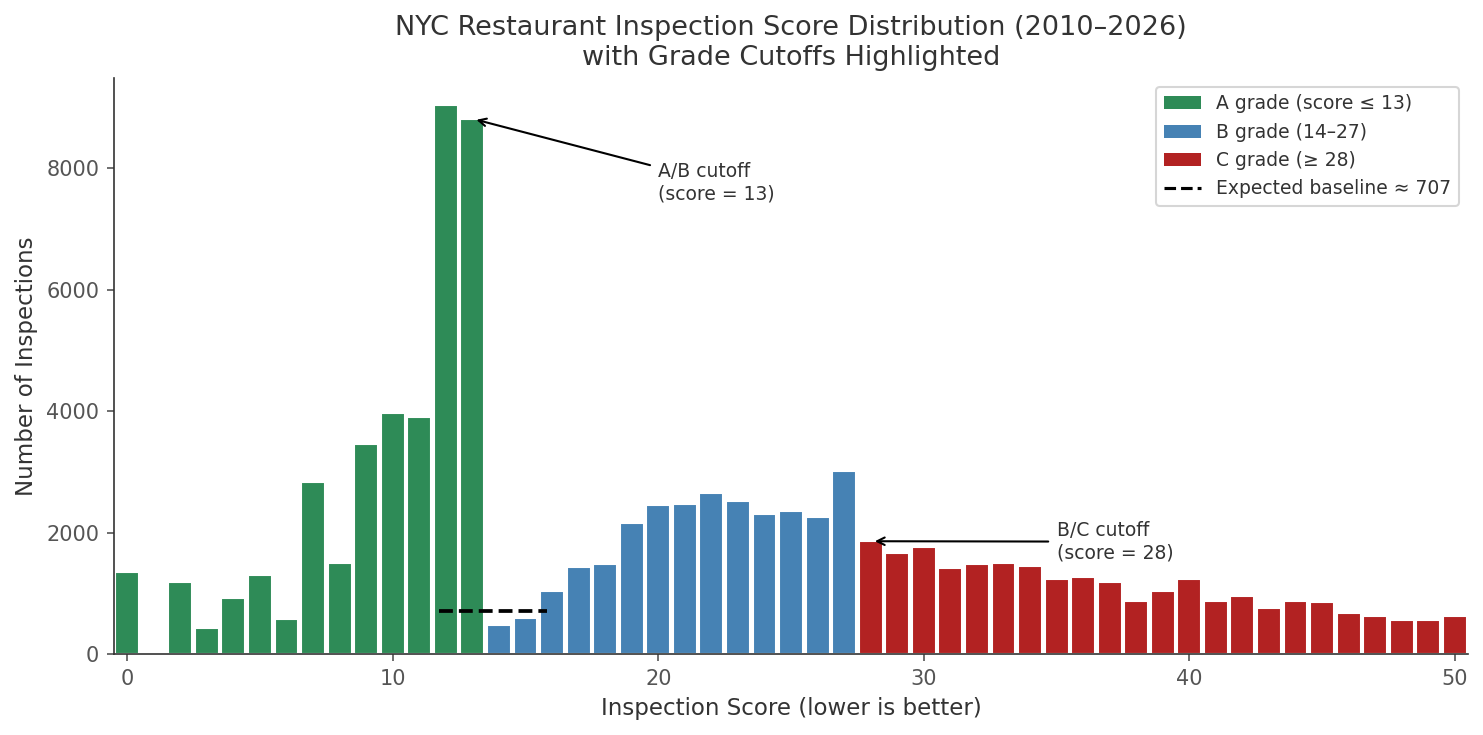
\includegraphics[width=\columnwidth]{fig1_score_distribution}
  \caption{Inspection score distribution (2010--2026). Green bars are
    A-grade inspections; blue are B; red are C. The dashed line shows
    the expected flat baseline near the A/B cutoff.}
  \label{fig:score_dist}
\end{figure}

The chi-square test is conclusive. Observed inspections at scores 12--13
total 17,863, against an expected 3,033 under a flat distribution. This
is a surplus of 14,830 inspections, or $+489\%$ above expectation
($\chi^2 = 30{,}792$, $p \approx 0$). Wellington's 2014 finding has not
faded. Figure~\ref{fig:bump} provides a zoomed view centered on the A/B
boundary.

\begin{figure}[h]
  \centering
  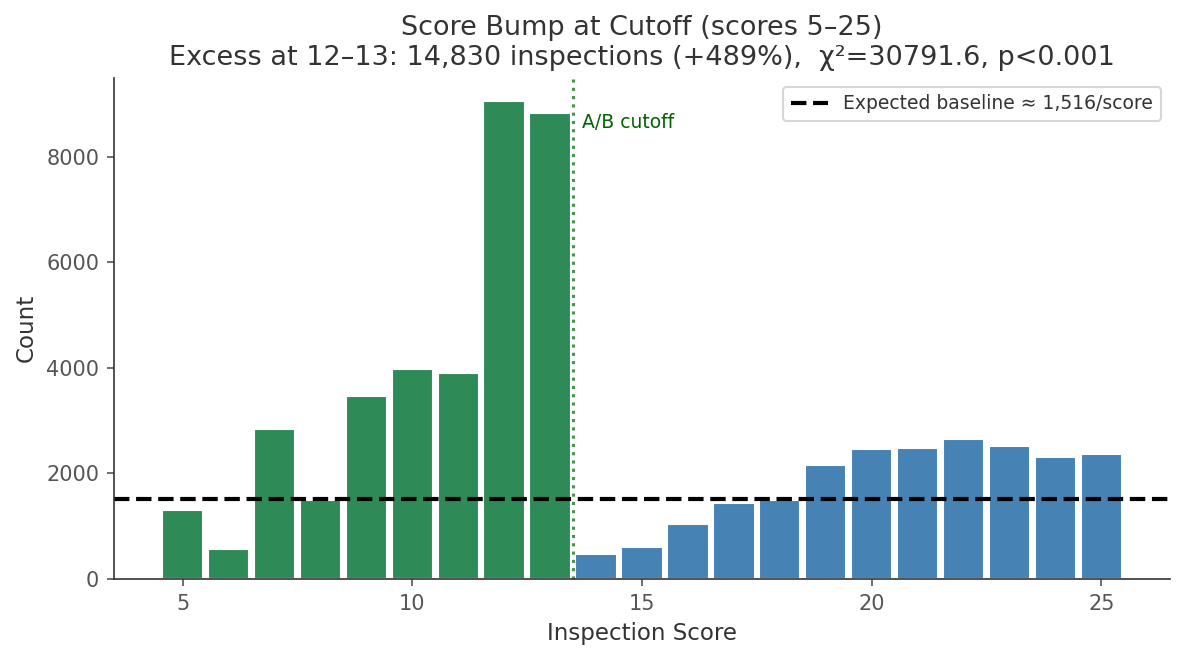
\includegraphics[width=\columnwidth]{fig2_bump_test}
  \caption{Zoomed view of scores 5--25. The dashed line shows the
    expected flat baseline. The spike at 12--13 represents roughly
    15,000 inspections above what would be expected under uniform grading.}
  \label{fig:bump}
\end{figure}

\subsection{Inspection Scores Have Worsened Substantially}

Figure~\ref{fig:temporal} shows mean initial-cycle inspection scores from
2015 to 2025, after deduplicating to one observation per inspection
event. The mean score increased from 11.3 in 2015 to 19.0 in 2025. A
simple linear regression estimates the rate of increase at 0.87 points
per year ($R^2 = 0.91$, $p < 0.001$). At this pace, the average
restaurant has shifted from comfortably earning an A on an initial
inspection in 2015 to scoring squarely in B-grade territory by 2025.

\begin{figure}[h]
  \centering
  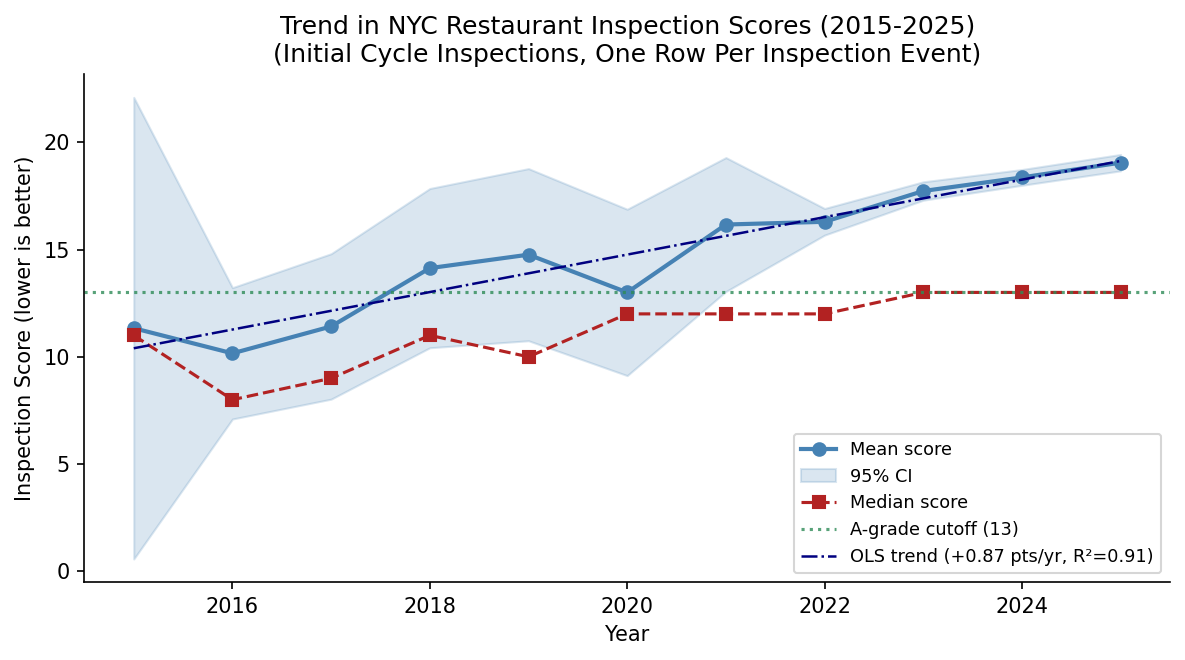
\includegraphics[width=\columnwidth]{fig3_temporal_trend}
  \caption{Mean and median inspection score by year (initial-cycle
    inspections only, one row per inspection event). The green dotted
    line marks the A-grade cutoff at 13.}
  \label{fig:temporal}
\end{figure}

The causes of this trend are not clear from the data alone. Possible
explanations include genuine deterioration in restaurant hygiene,
increased inspection stringency, changes in the restaurant population, or
some combination. Disentangling these explanations would require inspector
and restaurant fixed effects, which is left for future work.

\subsection{Borough and Cuisine Have Modest but Significant Effects}

Figure~\ref{fig:boro_cuisine} shows score distributions by borough and
by cuisine hypercategory. Manhattan restaurants score best (median 19),
followed by the Bronx and Brooklyn (both median 20), with Queens scoring
worst (median 22). These differences are present but modest in absolute
terms.

\begin{figure}[h]
  \centering
  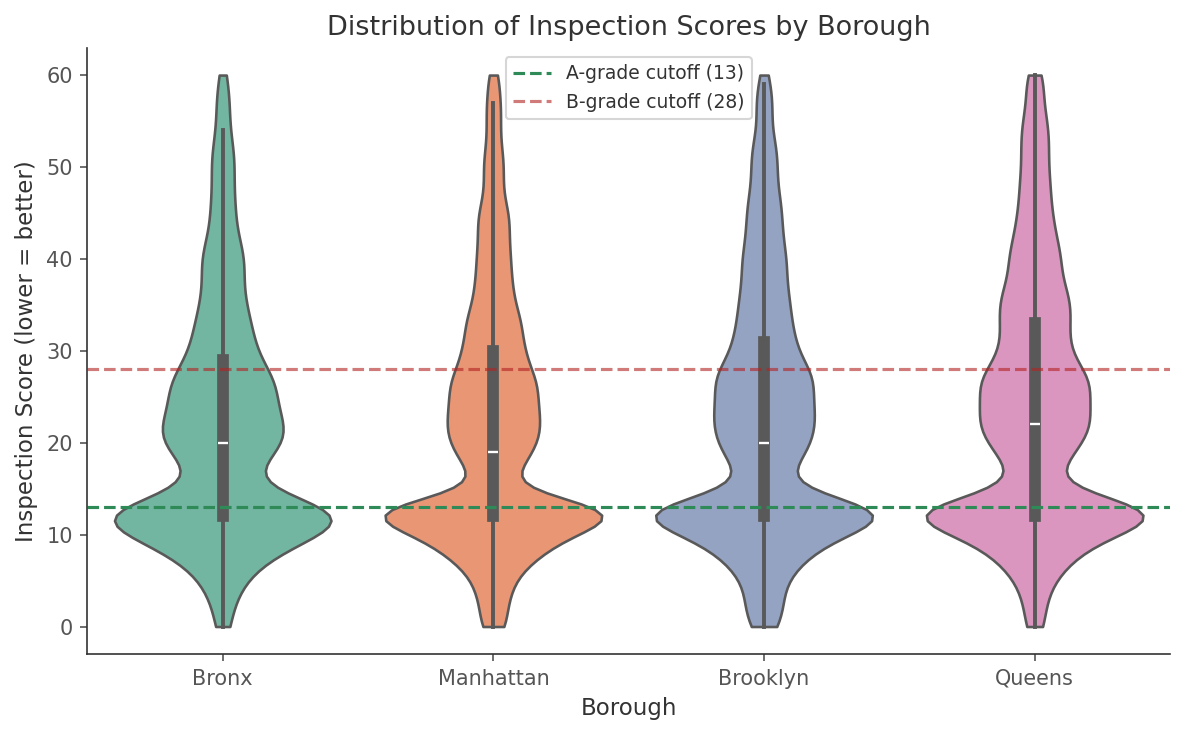
\includegraphics[width=\columnwidth]{fig4_score_by_borough}
  \caption{Score distributions by borough. Lower is better. Medians
    range from 19 (Manhattan) to 22 (Queens).}
  \label{fig:boro_cuisine}
\end{figure}

The two-way blocked ANOVA on $n = 30$ observations per cell confirms
these patterns. Cuisine hypercategory is a significant predictor
($F(9,1160) = 4.12$, $p < 0.001$), as is the hypercategory-by-borough
interaction ($F(27,1160) = 1.54$, $p = 0.038$). Borough alone is only
marginally significant ($F(3,1160) = 2.25$, $p = 0.081$). Effect sizes
are modest: the total residual variance ($SS_\text{res} = 482{,}194$)
dwarfs the variance attributable to borough and cuisine combined
($SS_\text{model} = 35{,}521$), suggesting that individual restaurant
practices explain far more of the outcome than geography or cuisine type.

\subsection{Violation Types Vary Significantly Across Boroughs}

Figure~\ref{fig:heatmap} shows the rate of each violation category by
borough, expressed as a percentage of all inspections in that borough.
The chi-square test strongly rejects independence between violation type
and borough ($\chi^2 = 678.2$, $df = 66$, $p \approx 2 \times 10^{-102}$).

\begin{figure}[h]
  \centering
  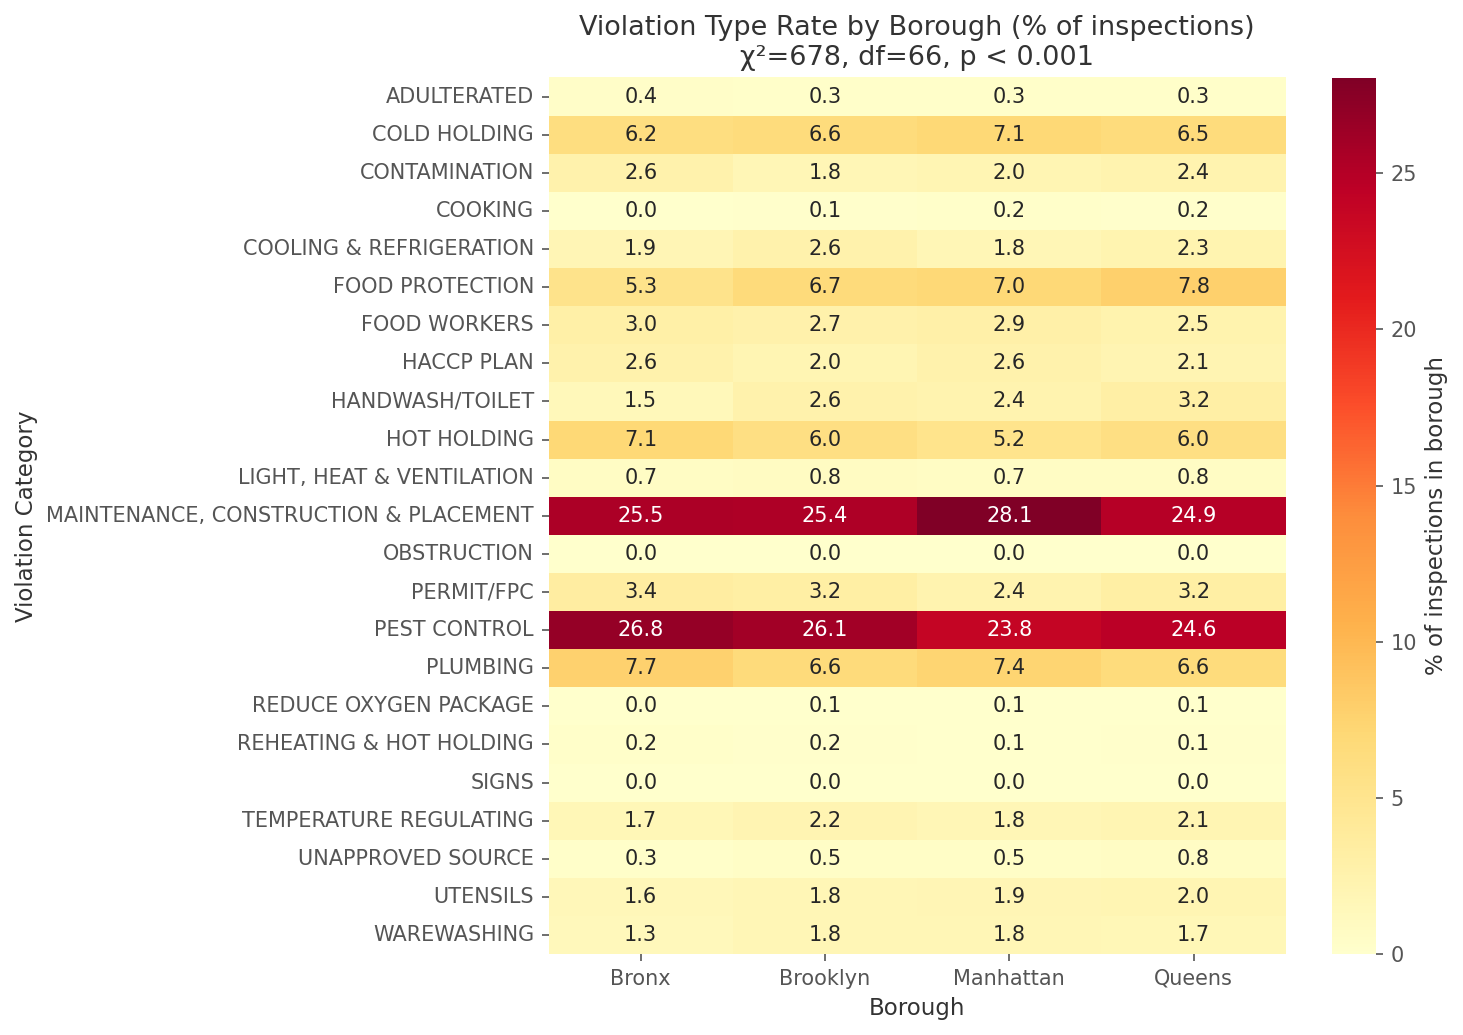
\includegraphics[width=\columnwidth]{fig5_violation_by_borough}
  \caption{Violation category rates by borough (\% of inspections).
    Darker cells indicate higher violation rates. Pest Control and
    temperature-related violations show the strongest geographic
    variation.}
  \label{fig:heatmap}
\end{figure}

Pest Control violations are more concentrated in the Bronx relative to
other boroughs. Cooling and Refrigeration violations are elevated in
Manhattan. Queens and Brooklyn show higher rates of Hot Holding
violations. These patterns likely reflect differences in restaurant type,
building infrastructure, and neighborhood environment rather than
inspection rigor alone, though the data cannot distinguish between these
explanations.

\subsection{Pre-Inspection Features Cannot Reliably Predict Grade}

The logistic regression using only pre-inspection features achieves an
AUC of 0.60 and an accuracy of 59.4\% on the held-out test set
(Table~\ref{tab:model_compare}). Both figures are barely above a
baseline classifier. The ROC curve is shown in Figure~\ref{fig:roc}.

\begin{table}[h]
  \centering
  \small
  \caption{Predictive model performance.}
  \label{tab:model_compare}
  \begin{tabular}{lcc}
    \toprule
    Model & AUC & Accuracy \\
    \midrule
    Pre-inspection features & 0.60 & 59.4\% \\
    \bottomrule
  \end{tabular}
\end{table}

\begin{figure}[h]
  \centering
  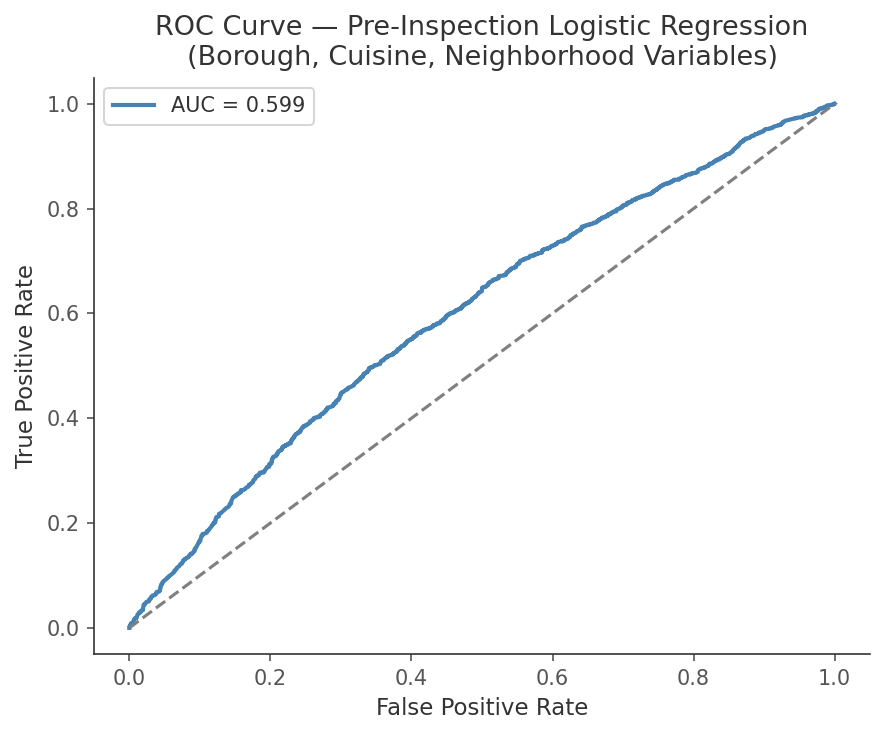
\includegraphics[width=0.85\columnwidth]{fig7_roc_curve}
  \caption{ROC curve for the pre-inspection logistic regression.
    An AUC near 0.60 indicates limited predictive power from borough,
    cuisine, and neighborhood variables alone.}
  \label{fig:roc}
\end{figure}

This near-chance performance has a clear interpretation: knowing where a
restaurant is located, what cuisine it serves, and how wealthy its
neighborhood is tells us very little about whether it will pass
inspection. Restaurant-level practices and management quality appear to
drive outcomes far more than contextual factors.

% ============================================================
\section{Model Validation}
% ============================================================

The predictive logistic regression was evaluated on a stratified 80/20
hold-out split, with standardization fit only on training data. No
information from the test set influenced model training. The modest AUC
of 0.60 reflects the genuine difficulty of predicting inspection outcomes
from pre-inspection characteristics rather than any deficiency in the
modeling approach.

For the ANOVA, we used balanced sampling across cells ($n = 30$ per
cell) to avoid the problem common in large observational datasets where
even negligible effect sizes produce highly significant $p$-values. The
results should be interpreted with effect sizes in mind rather than
$p$-values alone. Residual variance far exceeds the variance explained by
the model terms, placing clear limits on how much the between-group
differences matter practically.

The chi-square tests for the bump and the violation-by-borough analysis
use the full dataset and are therefore extremely well-powered. Effect
sizes in both cases are substantive: the 489\% excess at the grade
boundary is not a statistical artifact, and the geographic variation in
violation types is pronounced enough to be visible in the raw heatmap.

% ============================================================
\section{Conclusion}
% ============================================================

Four findings stand out from this analysis.

Grade-boundary leniency is real and has not diminished since Wellington's
2014 report. Nearly 15,000 inspections appear at scores 12--13 in excess
of what a fair distribution would predict. The NYC Health Department's
denial notwithstanding, the pattern in the data is striking and
consistent.

Inspection scores have worsened materially over the past decade. The
mean initial-inspection score rose by roughly 0.87 points per year from
2015 to 2025, moving from A-grade territory to solidly B-grade territory.
Whether this reflects actual deterioration in restaurant conditions or a
shift in inspection behavior is an important open question.

Violation types are not geographically uniform. Different boroughs show
distinct violation profiles, with Pest Control violations elevated in the
Bronx and temperature-related violations more prevalent in Manhattan and
outer boroughs. This geographic heterogeneity is highly statistically
significant and may be useful for targeted public health outreach.

Finally, context does not predict outcomes. With an AUC of 0.60, knowing
a restaurant's borough, cuisine, and neighborhood income cannot
meaningfully forecast whether it will earn an A. This reinforces the
conclusion from the ANOVA: most of the variation in inspection scores is
within-group, driven by factors specific to individual restaurants rather
than their broader context.

Future work could examine whether the grade-boundary spike varies by
borough or inspector team, or test whether the temporal worsening trend
persists after controlling for changes in the restaurant population.

% ============================================================
\appendix
\section*{Appendix A: Literature Review}
% ============================================================

% TODO: paste in HW2 literature review

% ============================================================
\section*{Appendix B: ANOVA Table}
% ============================================================

\begin{table}[h]
  \centering
  \small
  \caption{Two-way ANOVA results ($n = 30$ per cell, Bronx and African
    cuisine as baselines, Staten Island and Dietary Style excluded).}
  \label{tab:anova}
  \begin{tabular}{lrrrl}
    \toprule
    Term & Df & $F$ & $p$ & \\
    \midrule
    Hypercategory & 9 & 4.12 & $<0.001$ & *** \\
    Borough & 3 & 2.25 & 0.081 & . \\
    Hypercategory $\times$ Borough & 27 & 1.54 & 0.038 & * \\
    Residuals & 1160 & & & \\
    \bottomrule
    \multicolumn{5}{l}{\small Signif.: *** $p<0.001$, * $p<0.05$, . $p<0.1$}
  \end{tabular}
\end{table}

% ============================================================
\section*{Appendix C: Additional Figures}
% ============================================================

\begin{figure}[h]
  \centering
  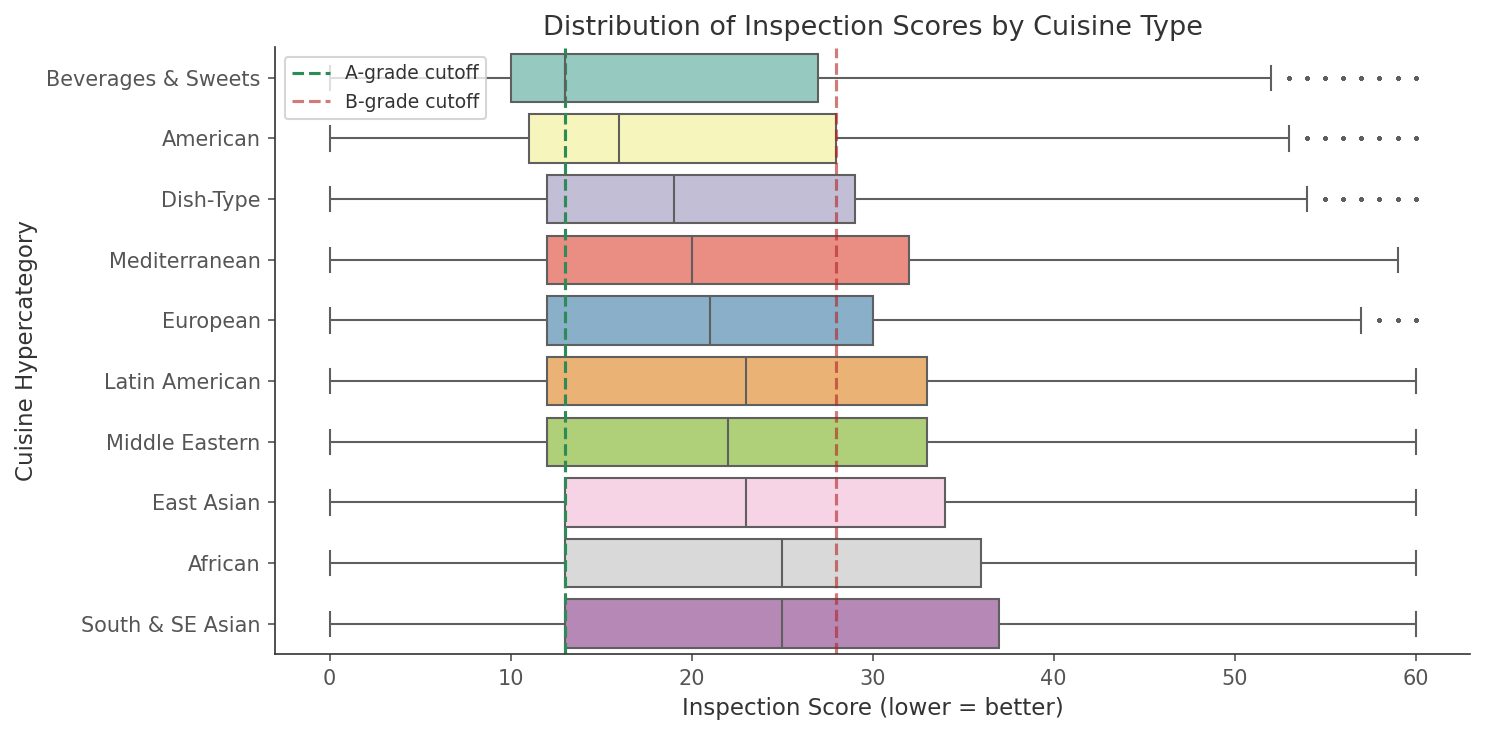
\includegraphics[width=\columnwidth]{fig6_score_by_cuisine}
  \caption{Score distributions by cuisine hypercategory. African and
    European restaurants score best on average; Dish-Type and Beverages
    \& Sweets score worst.}
\end{figure}

\begin{figure}[h]
  \centering
  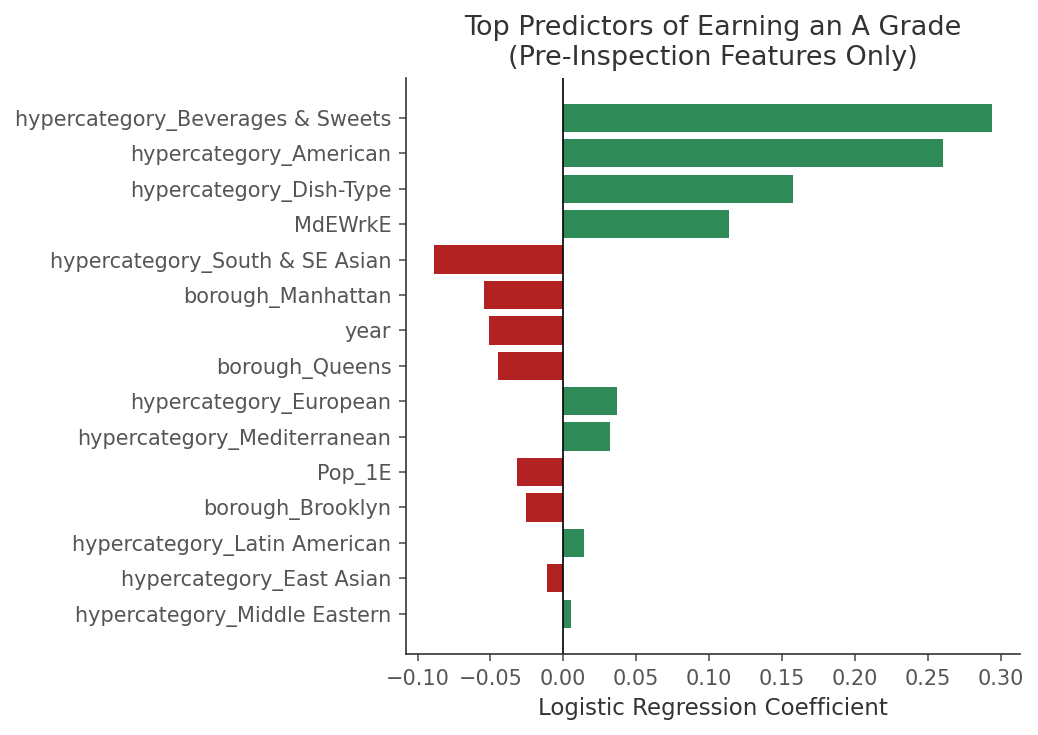
\includegraphics[width=\columnwidth]{fig8_coef_plot}
  \caption{Top 15 coefficients from the pre-inspection logistic
    regression. Green indicates positive association with earning an A;
    red indicates negative association. No predictor has a large
    coefficient, consistent with the low AUC.}
\end{figure}

% ============================================================
\section*{Appendix D: Code}
% ============================================================

Python analysis code is in \texttt{new\_analysis.py}. The R analysis
and ANOVA are in \texttt{group\_analysis.Rmd}. Both files are submitted
alongside this report.

\begin{thebibliography}{9}
\bibitem{wellington2014}
  Wellington, B. (2014).
  \textit{Think NYC Restaurant Grading is Flawed? Here's the Proof.}
  I Quant NY.
  \url{https://iquantny.tumblr.com/post/76928412519}
\end{thebibliography}

\end{document}
